\documentclass[pdflatex,compress]{beamer}

\usetheme[darktitle,framenumber,totalframenumber]{UniversiteitAntwerpen}
%\usetheme[light,framenumber,totalframenumber]{UniversiteitAntwerpen}

\usefonttheme[onlymath]{serif}
\usepackage{lipsum}
\setbeamertemplate{caption}[numbered]
\beamertemplatenavigationsymbolsempty

\usepackage[
backend=biber,
style=authoryear,
]{biblatex}
\addbibresource{bibliography.bib}

% For wrapping text in tables
\usepackage{colortbl}

% For advanced caption options, especially making some captions smaller
\usepackage{caption}

% To draw stuff
\usepackage{tikz}

% To outsource plots
\usepackage{standalone}

% To center captions
\usepackage[justification=centering]{caption}

% So we can include the standalones
\usepackage{pgfplots}
% To get rid of annoying "unsuitable tick labels; missing features" warning
\pgfplotsset{compat=1.16}

% For bold math characters
\usepackage{bm}

% For math stuff, e.g. align
\usepackage{amsmath}

% For quotations
\usepackage{csquotes}

% Graphviz plots in latex
\usepackage[pdf]{graphviz}

% To make \parencite use brackets instead of braces
\DeclareCiteCommand{\parencite}
  {\usebibmacro{prenote}}
  {\usebibmacro{citeindex}%
   \printtext[bibhyperref]{[\usebibmacro{cite}]}}
  {\multicitedelim}
  {\usebibmacro{postnote}}

\title{Building a network without backprop}
%\subtitle{This is a dummy subti}

\author{Bernhard Gstrein}

\begin{document}

\maketitle

\AtBeginSection[]{}

\begin{frame}
	\frametitle{Background/Motivation}
	\begin{itemize}[<+->]
		\item For learning neural networks, backpropagation is almost exclusively used
			\vspace{1em}
		\item Our goal: building a \enquote{network} without backprop
			\begin{itemize}
				\item Using local search, SAT solving, etc.
				\item Logic synthesis; input: goals and constraints, output: network structure
			\end{itemize}
			\vspace{1em}
		\item \parencite{chatterjee2018learning} describes a scheme to build something similar to a neural network without backprop
			\begin{itemize}
				\item Basic idea: lookup tables (\enquote{luts})
				\item Some properties of neural networks are promiment in lut networks too
			\end{itemize}
	\end{itemize}
\end{frame}

\AtBeginSection[]
{
  \begin{frame}
    \frametitle{Table of Contents}
    \tableofcontents[currentsection]
  \end{frame}
}

\begin{frame}
	\frametitle{Table of Contents}
\tableofcontents
\end{frame}

\section{Single lookup table ("lut")}

\begin{frame}
	\frametitle{What is a lookup table (lut)?}
		\vspace{1em}
		\small
		\begin{minipage}{.95\linewidth}\centering
			\begin{table}[]
			\begin{tabular}{lccclc}
																 & \multicolumn{3}{c}{$\bm{X}$}                                                    &                       & \multicolumn{1}{c}{$y$}          \\
																 & Lives in water         & Has eyes               & Has limbs              &                       & \multicolumn{1}{c}{Vertebrate} \\ \cline{2-4} \cline{6-6} 
			\multicolumn{1}{l|}{$\bm{x}_1$} & \multicolumn{1}{c|}{0} & \multicolumn{1}{c|}{1} & \multicolumn{1}{c|}{1} & \multicolumn{1}{l|}{} & \multicolumn{1}{c|}{1}         \\ \cline{2-4} \cline{6-6} 
			\multicolumn{1}{l|}{$\bm{x}_2$} & \multicolumn{1}{c|}{1} & \multicolumn{1}{c|}{1} & \multicolumn{1}{c|}{0} & \multicolumn{1}{l|}{} & \multicolumn{1}{c|}{1}         \\ \cline{2-4} \cline{6-6} 
			\multicolumn{1}{l|}{$\bm{x}_3$} & \multicolumn{1}{c|}{1} & \multicolumn{1}{c|}{0} & \multicolumn{1}{c|}{0} & \multicolumn{1}{l|}{} & \multicolumn{1}{c|}{0}         \\ \cline{2-4} \cline{6-6} 
			\end{tabular}
			\end{table}
		\end{minipage}
	\centering
	Model for classification of animals into vertebrates/invertebrates
	\normalfont
	\vspace{1em}
	\begin{itemize}
		\item<2-> We must binarize the features and labels
		\item<3-> We must limit the complexity
			\begin{itemize}
				\item<4-> Suppose we have 784 columns $\rightarrow$ \, $2^{784} \propto 10^{236}$
			\end{itemize}
	\end{itemize}
\end{frame}



\begin{frame}
	\frametitle{Preprocessing data}
	\begin{itemize}[<+->]
		\item MNIST dataset: 28x28 images of handwritten digits (0-9)
		\item We unroll the images: $28 \cdot 28 = 784$
		\item We map the values: $[0,255] \rightarrow [0,1]$
		\item We binarize the data using the operator $>0.5$
			\vspace{1em}
		\item Labels: $y=0$ (numbers 0-4), $y=1$ (numbers 5-9)
	\vspace{1em}
		\item We end up with
		\begin{itemize}
			\item Features $\bm{X}$: matrix of shape $(N, 784)$, boolean entries
			\item Labels $y$: vector of shape $(N,)$, boolean entries
		\end{itemize}
	\end{itemize}
\end{frame}

\begin{frame}
	\frametitle{A single lut}
	\begin{itemize}
		\item<1-> Every example is an instance of a \enquote{bit pattern} (e.g. $\bm{x}=10$) and has a label (e.g. $y=1$)
		\item<2-> We need a classification for each bit pattern: $f(00)=\,?$, $f(01)=\,?$, $f(10)=\,?$, $f(11)=\,?$
		\item<3-> For each bit pattern in $\bm{X}$, we cound how many times $y=0$ and $y=1$
	\end{itemize}
	\begin{align*}\onslide<4->{
		f(\text{bit pattern}) =
		\begin{cases}
			0 & \text{if} \hspace{1em} \sum\limits_{y=0} > \sum\limits_{y=1} \\
			1 & \text{if} \hspace{1em} \sum\limits_{y=0} < \sum\limits_{y=1} \\
			\text{rand}(0,1) & \text{if} \hspace{1em} \sum\limits_{y=0} = \sum\limits_{y=1}
		\end{cases}
	}
	\end{align*}
\end{frame}

\begin{frame}
	\frametitle{A single lut: example}
	\small
		\begin{minipage}{.95\linewidth}\centering
			\onslide<1->{
			\begin{minipage}[b]{.2\linewidth}\centering
				Training set
				\begin{align*}
					\begin{array}{cc}
						\bm{X}                         & y                      \\ \hline
						\multicolumn{1}{|c|}{000} & \multicolumn{1}{c|}{0} \\ \hline
						\multicolumn{1}{|c|}{000} & \multicolumn{1}{c|}{1} \\ \hline
						\multicolumn{1}{|c|}{000} & \multicolumn{1}{c|}{1} \\ \hline
						\multicolumn{1}{|c|}{001} & \multicolumn{1}{c|}{1} \\ \hline
						\multicolumn{1}{|c|}{100} & \multicolumn{1}{c|}{0} \\ \hline
						\multicolumn{1}{|c|}{110} & \multicolumn{1}{c|}{0} \\ \hline
						\multicolumn{1}{|c|}{110} & \multicolumn{1}{c|}{1} \\ \hline
					\end{array}
				\end{align*}
			\end{minipage}
		}
		\onslide<2->{
			\begin{minipage}[b]{.4\linewidth}\centering
				\begin{align*}
					\begin{array}{ccc}
						\text{bit pattern}        & \sum\limits_{y=0}      & \multicolumn{1}{l}{\sum\limits_{y=1}} \\ \hline
						\multicolumn{1}{|c|}{000} & \multicolumn{1}{c|}{1} & \multicolumn{1}{c|}{2}                \\ \hline
						\multicolumn{1}{|c|}{001} & \multicolumn{1}{c|}{0} & \multicolumn{1}{c|}{1}                \\ \hline
						\multicolumn{1}{|c|}{010} & \multicolumn{1}{c|}{0} & \multicolumn{1}{c|}{0}                \\ \hline
						\multicolumn{1}{|c|}{011} & \multicolumn{1}{c|}{0} & \multicolumn{1}{c|}{0}                \\ \hline
						\multicolumn{1}{|c|}{100} & \multicolumn{1}{c|}{1} & \multicolumn{1}{c|}{0}                \\ \hline
						\multicolumn{1}{|c|}{101} & \multicolumn{1}{c|}{0} & \multicolumn{1}{c|}{0}                \\ \hline
						\multicolumn{1}{|c|}{110} & \multicolumn{1}{c|}{1} & \multicolumn{1}{c|}{1}                \\ \hline
						\multicolumn{1}{|c|}{111} & \multicolumn{1}{c|}{0} & \multicolumn{1}{c|}{0}                \\ \hline
					\end{array}
				\end{align*}
			\end{minipage}
		}
		\onslide<3->{
			\begin{minipage}[b]{.3\linewidth}\centering
				\begin{align*}
					\begin{array}{cc}
						\text{bit pattern}        & f                  \\ \hline
						\multicolumn{1}{|c|}{000} & \multicolumn{1}{l|}{1}   \\ \hline
						\multicolumn{1}{|c|}{001} & \multicolumn{1}{l|}{1}   \\ \hline
						\multicolumn{1}{|c|}{010} & \multicolumn{1}{l|}{0^*} \\ \hline
						\multicolumn{1}{|c|}{011} & \multicolumn{1}{l|}{1^*} \\ \hline
						\multicolumn{1}{|c|}{100} & \multicolumn{1}{l|}{0}   \\ \hline
						\multicolumn{1}{|c|}{101} & \multicolumn{1}{l|}{1^*}  \\ \hline
						\multicolumn{1}{|c|}{110} & \multicolumn{1}{l|}{1^*}  \\ \hline
						\multicolumn{1}{|c|}{111} & \multicolumn{1}{l|}{0^*} \\ \hline
					\end{array}
				\end{align*}
			\end{minipage}
		}
		\end{minipage}
		\onslide<3->{
	\begin{minipage}[b]{.95\linewidth}
		\vspace{1em}
		\hspace*{0pt}\hfill $^*$: randomly chosen entries
	\end{minipage}
}
			\normalfont
\end{frame}


\section{Network of lookup tables ("luts")}

\begin{frame}
	\frametitle{A single neuron}
		\vspace{-110px}
	\begin{minipage}[b]{0.95\linewidth}
		\onslide<1->{
		\begin{minipage}[b]{0.45\linewidth}
			\centering
			Neural network
		\end{minipage}
	}
	\onslide<2->{
		\begin{minipage}[b]{0.45\linewidth}
			\centering
			\hspace{75px} Lut network
		\end{minipage}
	}
	\end{minipage}
	\onslide<1->{
		\begin{tikzpicture}[remember picture,overlay]
				\node[xshift=-9.5cm,yshift=-5.0cm] at (current page.north east) {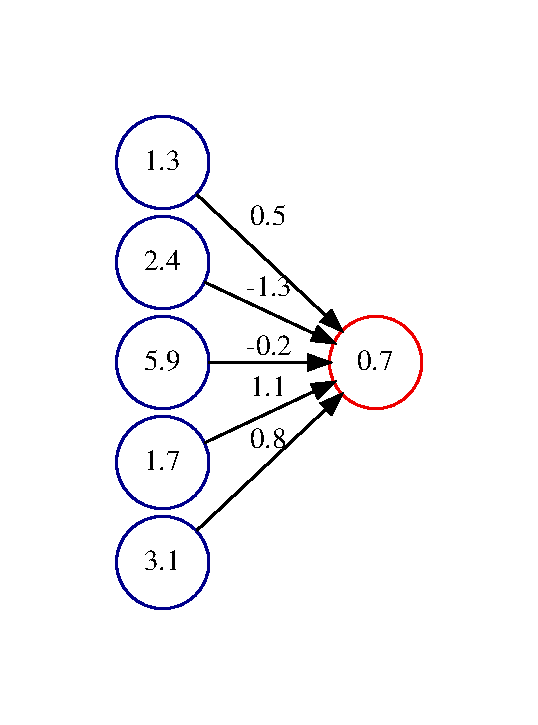
\includegraphics[width=120px,keepaspectratio]{images/single_neuron_nn.pdf}};
		\end{tikzpicture}
	}
	\onslide<2->{
		\begin{tikzpicture}[remember picture,overlay]
				\node[xshift=-3.3cm,yshift=-5.0cm] at (current page.north east) {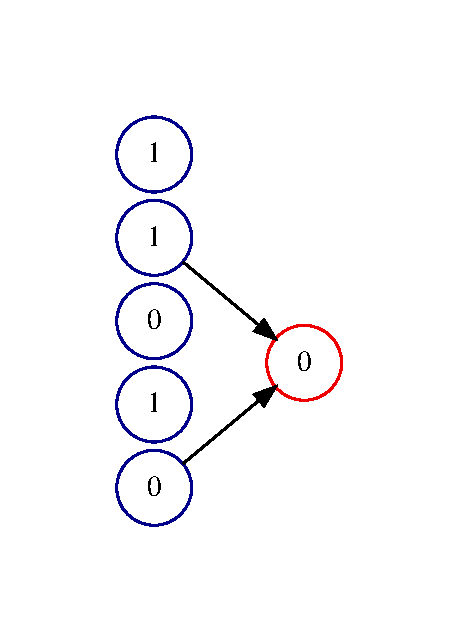
\includegraphics[width=120px,keepaspectratio]{images/single_neuron_lut.pdf}};
		\end{tikzpicture}
	}
		\onslide<1->{
			\begin{tikzpicture}[remember picture,overlay]
				\node[xshift=-9.1cm,yshift=-8.0cm] at (current page.north east) {
					\begin{minipage}{150px}
					\small$z=1.3 \cdot 0.5 - 2.4 \cdot 1.3 - 5.9 \cdot 0.2 + 1.7 \cdot 1.1 + 3.1 \cdot 0.8 = 0.7$
					\break
					$f(z) = \text{ReLU}(z) = \text{max}(0,z) = 0.7$
					\end{minipage}
				};
			\end{tikzpicture}
		}
		\onslide<2->{
			\begin{tikzpicture}[remember picture,overlay]
				\node[xshift=-2.0cm,yshift=-7.7cm] at (current page.north east) {
					\begin{minipage}{150px}
						\footnotesize
						\begin{table}[]
						\begin{tabular}{ll}
						Bit pattern & $f$ \\
						\hline 
						00          & 0 \\
						01          & 1 \\
						10          & 0 \\
						11          & 1
						\end{tabular}
						\end{table}
					\end{minipage}
				};
			\end{tikzpicture}
		}
\end{frame}

\begin{frame}
	\frametitle{Neural network - lut network: comparison}
		\vspace{-80px}
	\begin{minipage}[b]{0.95\linewidth}
		\onslide<1->{
		\begin{minipage}[b]{0.45\linewidth}
			\centering
			Neural network
		\end{minipage}
	}
	\onslide<2->{
		\begin{minipage}[b]{0.45\linewidth}
			\centering
			\hspace{75px} Lut network
		\end{minipage}
	}
	\end{minipage}
	\onslide<1->{
		\begin{tikzpicture}[remember picture,overlay]
				\node[xshift=-9.5cm,yshift=-6.1cm] at (current page.north east) {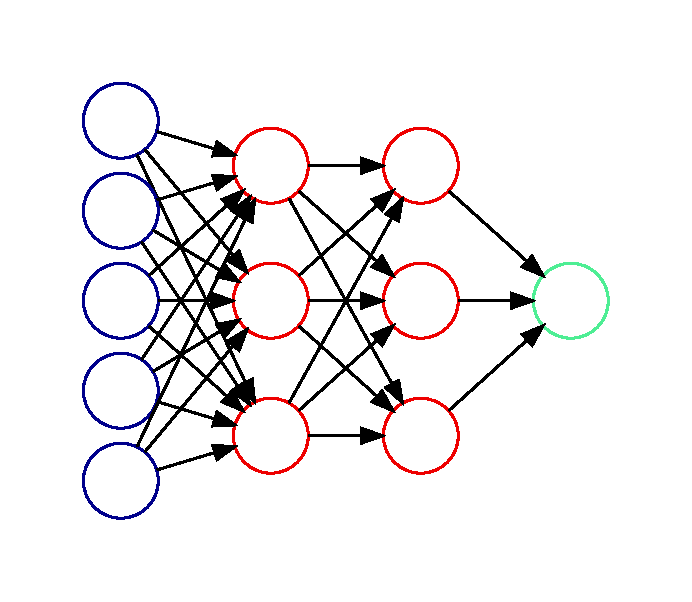
\includegraphics[width=180px,keepaspectratio]{images/FCNN.pdf}};
		\end{tikzpicture}
	}
	\onslide<2->{
		\begin{tikzpicture}[remember picture,overlay]
				\node[xshift=-3.3cm,yshift=-5.9cm] at (current page.north east) {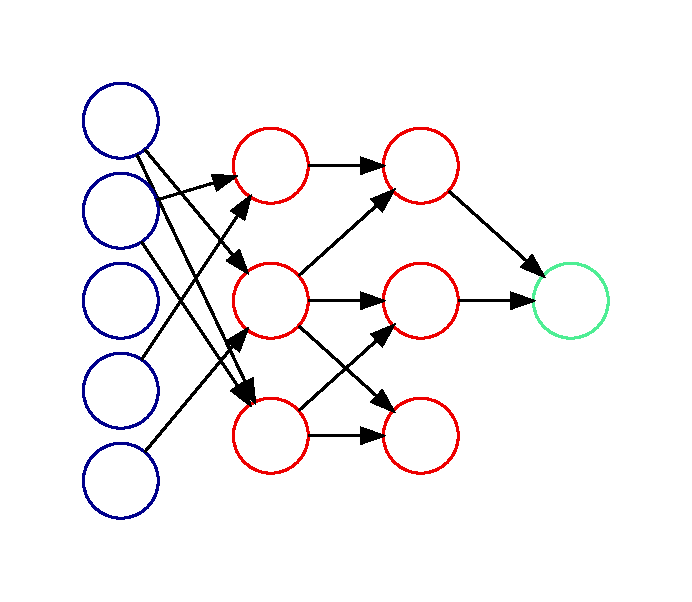
\includegraphics[width=180px,keepaspectratio]{images/lut.pdf}};
		\end{tikzpicture}
	}
\end{frame}

\mode<beamer>{
\begin{frame}
	\frametitle{Lut network: example}
		\begin{minipage}[b]{.98\linewidth}
			\centering
			\begin{minipage}[b]{.45\linewidth}
				\begin{table}[]
				\begin{tabular}{llll}
				bit pattern & $f_0$ & $f_1$ & $f_2$ \\ \hline
				00          & 1     & 1     & 1     \\
				01          & 0     & 0     & 1     \\
				10          & 1     & 0     & 0     \\
				11          & 0     & 1     & 0    
				\end{tabular}
				\end{table}
				\vspace{-1em}
			\end{minipage}
			\begin{minipage}[b]{.48\linewidth}
		\begin{tikzpicture}[remember picture,overlay]
				\node[xshift=-3.3cm,yshift=-5.0cm] at (current page.north east) {
					\includegraphics<1>[width=180px]{images/ex/00.pdf}%
					\includegraphics<2>[width=180px]{images/ex/01.pdf}%
					\includegraphics<3>[width=180px]{images/ex/02.pdf}%
					\includegraphics<4>[width=180px]{images/ex/03.pdf}%
				};
		\end{tikzpicture}
			\end{minipage}
		\end{minipage}
		\begin{tikzpicture}[remember picture,overlay] \node[xshift=-3.0cm,yshift=-3.4cm] at (current page.north east) {$f_0$}; \end{tikzpicture}
		\begin{tikzpicture}[remember picture,overlay] \node[xshift=-3.0cm,yshift=-5.3cm] at (current page.north east) {$f_1$}; \end{tikzpicture}
		\begin{tikzpicture}[remember picture,overlay] \node[xshift=-1.1cm,yshift=-4.4cm] at (current page.north east) {$f_2$}; \end{tikzpicture}
\end{frame}
}

\mode<handout>{
\begin{frame}
	\frametitle{Lut network: example}
		\begin{minipage}[b]{.98\linewidth}
			\centering
			\begin{minipage}[b]{.45\linewidth}
				\begin{table}[]
				\begin{tabular}{llll}
				bit pattern & $f_0$ & $f_1$ & $f_2$ \\ \hline
				00          & 1     & 1     & 1     \\
				01          & 0     & 0     & 1     \\
				10          & 1     & 0     & 0     \\
				11          & 0     & 1     & 0    
				\end{tabular}
				\end{table}
				\vspace{-1em}
			\end{minipage}
			\begin{minipage}[b]{.48\linewidth}
		\begin{tikzpicture}[remember picture,overlay]
				\node[xshift=-3.3cm,yshift=-5.0cm] at (current page.north east) {
					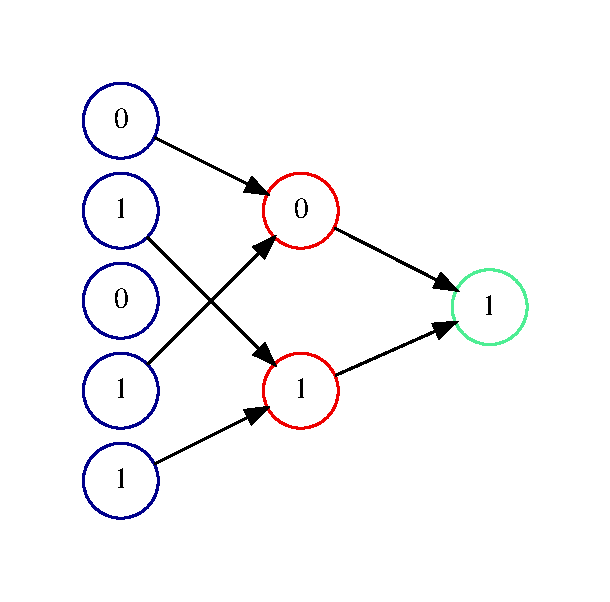
\includegraphics[width=180px]{images/ex/03.pdf}
				};
		\end{tikzpicture}
			\end{minipage}
		\end{minipage}
		\begin{tikzpicture}[remember picture,overlay] \node[xshift=-3.0cm,yshift=-3.4cm] at (current page.north east) {$f_0$}; \end{tikzpicture}
		\begin{tikzpicture}[remember picture,overlay] \node[xshift=-3.0cm,yshift=-5.3cm] at (current page.north east) {$f_1$}; \end{tikzpicture}
		\begin{tikzpicture}[remember picture,overlay] \node[xshift=-1.1cm,yshift=-4.4cm] at (current page.north east) {$f_2$}; \end{tikzpicture}
\end{frame}
}

\begin{frame}
	\frametitle{Training a network of luts}
		\begin{minipage}[b]{0.5\linewidth}
			\begin{itemize}[<+->]
			\item Lut network: layers are trained successively
				\vspace{1em}
				\item Random choice of $k$ columns for each lut
					\vspace{1em}
				\item Label vector is \textbf{always} $y$
		\end{itemize}
	\end{minipage}
		\begin{tikzpicture}[remember picture,overlay]
				\node[xshift=-3.3cm,yshift=-5.0cm] at (current page.north east) {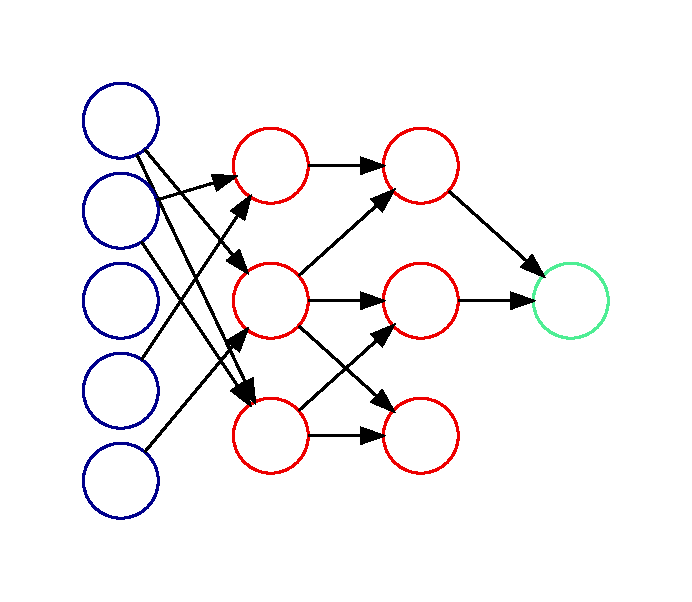
\includegraphics[width=180px,keepaspectratio]{images/lut.pdf}};
		\end{tikzpicture}
		\begin{tikzpicture}[remember picture,overlay] \node[xshift=-5.3cm,yshift=-2.7cm] at (current page.north east) {\small Input}; \end{tikzpicture}
		\begin{tikzpicture}[remember picture,overlay] \node[xshift=-1.2cm,yshift=-4.3cm] at (current page.north east) {\small Output}; \end{tikzpicture}
		\begin{tikzpicture}[remember picture,overlay] \node[xshift=-3.9cm,yshift=-3.1cm] at (current page.north east) {\small Hidden 1}; \end{tikzpicture}
		\begin{tikzpicture}[remember picture,overlay] \node[xshift=-2.3cm,yshift=-3.1cm] at (current page.north east) {\small Hidden 2}; \end{tikzpicture}
\end{frame}

\section{Experimental results from paper}

\begin{frame}
	\frametitle{First experiment}
	\begin{itemize}[<+->]
		\item Network with 5 hidden layers of 1024 luts and 1 lut in the output layer
			\vspace{1em}
		\item Each lut takes 8 inputs
			\vspace{1em}
		\item Training accuracy: 0.89
			\vspace{1em}
		\item Accuracy on held-out set: 0.87
			\vspace{1em}
		\item Results significantly above 0.5
	\end{itemize}
\end{frame}

\begin{frame}
	\frametitle{Network of luts: depth improves performance}
	\begin{figure}[ht]
		\centering
		\includestandalone[width=.5\linewidth]{standalone/depth_performance}
		\caption*{Training accuracy by layer for a network of 8-input lookup tables on Binary-MNIST. Each layer has 1024 luts except the last one which has only 1. Total height of error bars are two standard deviations.}
	\end{figure}
\end{frame}

\begin{frame}
	\frametitle{Network of luts}
	\begin{figure}
		\begin{minipage}[b]{.98\linewidth}
			\centering
				\begin{minipage}[b]{.48\textwidth}
				\centering
				\includestandalone[width=1\linewidth]{standalone/k_acc_real}
				\end{minipage}
				\begin{minipage}[b]{.48\textwidth}
				\centering
				\includestandalone[width=1\linewidth]{standalone/k_acc_rand}
				\end{minipage}
		\end{minipage}
	\caption*{Effect of varying lookup table size on Binary-MNIST. There are 5 hidden layers with 1024 luts per layer.}
	\end{figure}

\end{frame}

\section{Conclusion/outlook}

\begin{frame}
	\frametitle{Conclusion}
	\begin{itemize}[<+->]
	\item In the paper, there is also:
		\begin{itemize}
			\item More experiments with other datasets and other tasks
			\item Comparison of luts to other predictive models
		\end{itemize}
		\vspace{1em}
	\item Neural networks and lut networks share some properties:
		\begin{itemize}
			\item Depth improves performance
			\item There is generalization on real data
			\item Random data can be memorized
		\end{itemize}
		\vspace{1em}
	\item \textbf{The lut network is built without backprop and is able to perform non-trivial tasks}
\end{itemize}
\end{frame}

\begin{frame}
	\frametitle{Outlook}
	\begin{itemize}[<+->]
		\item We already wrote code that implements lut networks
			\begin{itemize}
				\item Recreate paper results for practical work?
			\end{itemize}
			\vspace{1em}
		\item Should we continue with luts?
			\vspace{1em}
		\item Building an AIG using local search/SAT solving sounds more interesting
	\end{itemize}
\end{frame}

\begin{frame}
\begin{figure}
\centering
\includegraphics[width=140px]{images/professorcat.jpg}
\end{figure}
\begin{center}
\huge Thank you for your attention!
\end{center}
\end{frame}

\section{References}

\begin{frame}
\frametitle{References}
\printbibliography
\end{frame}

\section{Appendix}

\begin{frame}
	\frametitle{Depth improves performance: Our results}
	\begin{figure}
		\begin{minipage}[b]{.98\linewidth}
			\centering
				\begin{minipage}[b]{.48\linewidth}
				\centering
				\includestandalone[width=1\linewidth]{standalone/depth_performance_title}
				\end{minipage}
				\begin{minipage}[b]{.48\linewidth}
				\centering
				\includestandalone[width=1\linewidth]{standalone/depth_performance_my}
				\end{minipage}
		\end{minipage}
		\caption*{\tiny Training accuracy by layer for a network of 8-input lookup tables on Binary-MNIST. Each layer has 1024 luts except the last one which has only 1. Total height of error bars are two standard deviations. We can see that our results closely match the results from the paper.}
	\end{figure}
\end{frame}



\end{document}
